% -------------------------------------------------------------------- %
% -------------------------------------------------------------------- %
% -------------------------------------------------------------------- %

\documentclass[onecolumn,12pt]{article} % here we use the article class, rather than elsarticle

% -------------------------------------------------------------------- %
% -------------------------------------------------------------------- %
% -------------------------------------------------------------------- %

\usepackage[square,numbers,sort&compress,comma]{natbib}

\usepackage{amsmath}
\usepackage{amssymb}
\usepackage{xcolor}
\usepackage{caption}
\usepackage{graphicx}
\usepackage{latexsym}
\usepackage{times}
\usepackage{dblfloatfix}

% -------------------------------------------------------------------- %
% -------------------------------------------------------------------- %
% -------------------------------------------------------------------- %

\topmargin - 12pt % might need to be set to 0pt for some installations
\oddsidemargin 32pt
\textheight 610pt
\textwidth 408pt
\columnsep 24pt

% -------------------------------------------------------------------- %
% -------------------------------------------------------------------- %
% -------------------------------------------------------------------- %

\def\thepage{}

\renewenvironment{abstract}%
              {% - begin definition
               \small% - select font
               {\bfseries \abstractname}% - select font
               \par% - end a paragraph (skip \parsep)
               \vspace{10pt}% - add vertical space
              }% - complete definition

\renewcommand\abstractname{Abstract}

\newcommand{\nomenclature}% - name of command
              [1]% - number of arguments
              {% - begin definition
               \bgroup% - begin a local group
               \flushleft% - turn on flushleft option
               \small\bf% - select font
               #1% - insert title text
               \par% - end a paragraph (skip \parsep)
               \egroup% - terminate local group
              }% - complete definition

\renewcommand{\section}% - name of command
              [1]% - number of arguments
              {% - begin definition
               \bgroup% - begin a local group
               \flushleft% - turn on flushleft option
               \small\bf% - select font
               \stepcounter{section}% - increment counter
               \arabic{section}. #1% - insert title text
               \par% - end a paragraph (skip \parsep)
               \egroup% - terminate local group
              }% - complete definition

\renewcommand{\subsection}% - name of command
              [1]% - number of arguments
              {% - begin definition
               \bgroup% - begin a local group
               \flushleft% - turn on flushleft option
               \small\em% - select font
               \stepcounter{subsection}% - increment counter
               \arabic{section}.% - insert title text
               \arabic{subsection}. #1% - insert title text
               \par% - end a paragraph (skip \parsep)
               \egroup% - terminate local group
              }% - complete definition

\renewcommand{\subsubsection}% - name of command
              [1]% - number of arguments
              {% - begin definition
               \bgroup% - begin a local group
               \flushleft% - turn on flushleft option
               \small\em% - select font
               \stepcounter{subsubsection}% - increment counter
               \arabic{section}.% - insert title text
               \arabic{subsection}.% - insert title text
               \arabic{subsubsection}. #1% - insert title text
               \par% - end a paragraph (skip \parsep)
               \egroup% - terminate local group
              }% - complete definition

  \newcommand{\acknowledgement}% - name of command
              [1]% - number of arguments
              {% - begin definition
               \bgroup% - begin a local group
               \flushleft% - turn on flushleft option
               \small\bf% - select font
               #1% - insert title text
               \par% - end a paragraph (skip \parsep)
               \egroup% - terminate local group
              }% - complete definition

  \newcommand{\sectionbib}% - name of command
              [1]% - number of arguments
              {% - begin definition
               \bgroup% - begin a local group
               \flushleft% - turn on flushleft option
               \small\bf% - select font
               #1% - insert title text
               \par% - end a paragraph (skip \parsep)
               \egroup% - terminate local group
              }% - complete definition
              
\newcommand{\beginsupplement}{%
        \setcounter{table}{0}
        \renewcommand{\thetable}{S\arabic{table}}%
        \setcounter{figure}{0}
        \renewcommand{\thefigure}{S\arabic{figure}}%
     }
     
\renewcommand\figurename{Fig.}
\renewcommand{\captionsize}{\footnotesize}
\setlength\abovecaptionskip{0pt}
\setlength\belowcaptionskip{0pt}

\renewcommand\bibsection{\sectionbib{\refname}}

\setlength\bibsep{0pt}

\pagenumbering{arabic}

% -------------------------------------------------------------------- %
% -------------------------------------------------------------------- %
% -------------------------------------------------------------------- %

\begin{document}
\beginsupplement
\title{\LARGE Mitigation of thermoacoustic instability in \\
                     a turbulent combustor via self-coupling}

\author{{\large Ankit Sahay$^{*}$, Author 2 full name$$, Author 3 full name$$, $\ldots$ (13/15)}\\[10pt]
        {\footnotesize \em $^a$Indian Institute of Technology Madras, Chennai 600036, India }\\[-5pt]}

\date{}

% -------------------------------------------------------------------- %
% -------------------------------------------------------------------- %
% -------------------------------------------------------------------- %

\small
\baselineskip 12pt


\clearpage

\section{Supplementary material} \addvspace{16pt}

\subsection{Detection of chaos in acoustic pressure oscillations during the state of complete suppression} \addvspace{10pt}

\begin{figure*}[h]
\centering
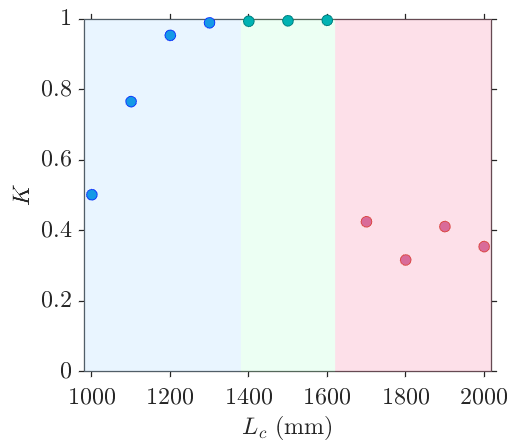
\includegraphics[width=0.5\textwidth]{chaos_test_p.png}
\caption{The results on applying the 0–1 test for chaos for different lengths of the coupling tube. The values gradually increase with the increase in length of the coupling tube $L_c$, and eventually reach close to 1 during the state of complete suppression (red-shaded region). As $L_c$ is increased beyond the region of complete suppression, we observe a sudden drop in the $K$ values (green-shaded region), indicating loss of chaos. The internal diameter of the coupling tube is kept constant at 25.4 mm for all experiments.}
\label{chaos_fig}
\end{figure*}

To confirm the presence of chaos in the dynamics of acoustic pressure, observed during the state of complete suppression of large amplitude periodic oscillations (i.e., thermoacoustic instability) when the combustor is self-coupled at optimum lengths and diameters of the coupling tube, we perform the 0-1 test for chaos \cite{gottwald2004new}. This test has been previous used by Nair \textit{et al}. \cite{nair2013loss} to confirm chaos in the acoustic pressure fluctuations acquired during the state of stable operation (combustion noise). We will first present the mathematical details of the 0-1 test for chaos and then discuss the existence of chaos in the dynamics of acoustic pressure of the self-coupled combustor. 

Let us consider the input time series to be $\alpha(t)$. The first step is to compute the translation variables $r(n)$ and $s(n)$ such that \cite{gottwald2004new}
\begin{equation}
\begin{aligned}
    \textcolor{black}{r(n) = \sum_{j=1}^n \alpha(t) \ \text{cos} \ (tc)} \\[-1pt]
    \textcolor{black}{s(n) = \sum_{j=1}^n \alpha(t) \ \text{sin} \ (tc)}.
\end{aligned}
\end{equation}
Here, $n = 1,2,...,N$, where $N$ is the total number of data points in time series. For our analysis, we have selected the value of $c$ in the interval $(\pi/5, 4\pi/5)$\cite{nair2013loss}. The behavior of these two translation variables also makes it possible to determine whether there is chaos in the system. For periodic or quasiperiodic oscillations, these variables exhibit bounded behavior. However, for chaotic dynamics, their behavior is unbounded and irregular. The behavior of the trajectory in the $r(n)-s(n)$ plane for increasing $n$ can be computed with the help of modified mean square displacement $M(n)$ as follows:
\begin{equation}
\begin{aligned}
   M(n) = \frac{1}{N} \sum_{J=1}^n [\ (r(j+n)-r(j))^2+ (s(j+n)-s(j))^2] -\frac{1}{N}  \sum_{j=1}^n \alpha(t)  \frac{1- \text{cos} \ (jc)}{1-\text{cos} \ (c)})
\end{aligned}
\end{equation}

For chaotic oscillations, $M(n)$ shows an increasing monotonous trend with $n$, whereas it becomes almost constant for regular oscillations. With the help of linear regression, the asymptotic growth of the mean displacement is calculated as follows:
\begin{equation}
\centering
K = \lim_{n\to \infty} \frac{\log M(n)}{\log n}.
\end{equation}
The value of $K$ lies between 0 and 1. For a chaotic signal, $K$ takes a value close to 1, and for a regular signal, it approaches a value close to 0 \cite{gottwald2004new}. 

In Fig.\ref{chaos_fig}, we observe the intermediate value of $K$ in the region of intermediate suppression. With the increment in the length of connecting tube ($L_c$), we notice that the value of $K$ increases to 1 which confirms the presence of chaos in the system during the total suppression of thermoacoustic instability. However, with further increase in length, we again see the value of $K$ decreases more than 0.5, indicating loss of chaos when the combustor exhibits no suppression after it is self-coupled. The 0-1 test demonstrates that as the suppression of thermoacoustic instability increases in the system with change in the length in the coupling tube, the system becomes chaotic.  

\subsection{Spatial distribution of Rayleigh Index for different coupling lengths} \addvspace{10pt}

\begin{figure*}[h]
\centering
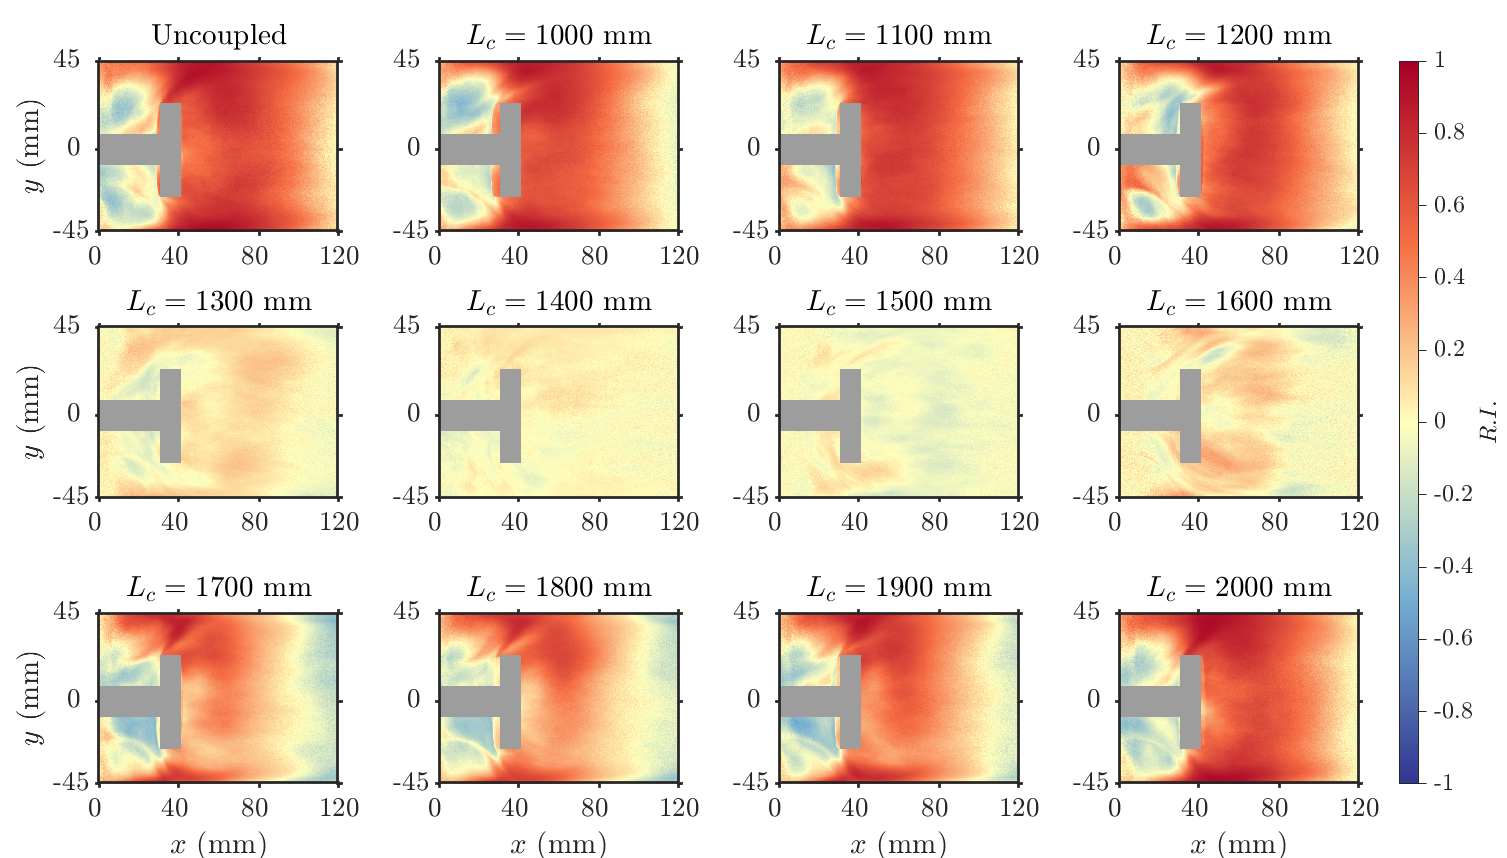
\includegraphics[width=1\textwidth]{rayleigh_index_plots.png}
\caption{Rayleigh index ($R.I.$) distribution for uncoupled and self-coupled combustor with coupling tubes of different lengths. The blue and red regions quantify the greater strength of acoustic power sinks and sources, respectively. The internal diameter of the coupling tube is kept constant at 25.4 mm for all self-coupled experiments. The Rayleigh index shows very high values downstream of the bluff body during thermoacoustic instability in an uncoupled state and during coupled state with low $L_c$ values. There is a significant change in the distribution of $R.I.$ for $L_c = 1300$ to $1600$ mm values ($L_c/L_{duct} \approx 1.5$, $L_{duct}$ = 1060 mm), where we observe very low $R.I.$ values throughout the combustor. }
\label{chaos_fig}
\end{figure*}





% -------------------------------------------------------------------- %
% -------------------------------------------------------------------- %
% -------------------------------------------------------------------- %

 \footnotesize
 \baselineskip 9pt

% -------------------------------------------------------------------- %
% -------------------------------------------------------------------- %
% -------------------------------------------------------------------- %

\bibliographystyle{pci}
\bibliography{PCI_LaTeX}

% -------------------------------------------------------------------- %
% -------------------------------------------------------------------- %
% -------------------------------------------------------------------- %

\newpage

\baselineskip 14pt

% -------------------------------------------------------------------- %
% -------------------------------------------------------------------- %
% -------------------------------------------------------------------- %

% -------------------------------------------------------------------- %
% -------------------------------------------------------------------- %
% -------------------------------------------------------------------- %

\end{document}

% -------------------------------------------------------------------- %
% -------------------------------------------------------------------- %
% -------------------------------------------------------------------- %
